\section{Results} \label{sec:rim:results}

In this section, we explore three key questions:

\textbf{How extensive are review reclassifications on Yelp?} Yelp presents most reviews as either ``Recommended'' or ``Not Recommended'', and Yelp moves reviews between those categories. However, Yelp does not discuss how frequently this movement occurs. Reclassifications are an indicator of the confidence Yelp has in its classifications, the challenging nature of the problem, the effort Yelp puts into updating its classifier, and may frustrate consumers and businesses.

\textbf{How do density and income impact reviews on Yelp?} Disparities in reviews in different regions
%\pmNote{vague phrasing}
are an important part of understanding equity on review platforms. For example, it could be possible that certain regions are disproportionately targeted by malicious reviews, or that Yelp's classifier is tuned towards a certain subset of regions.

\textbf{How do mask discussions and requirements impact businesses on Yelp?} With the ongoing COVID-19 pandemic, masks have been a controversial topic~\cite{pascual2021toxicity}, but how have mask requirements and mask discussion affected businesses?

For our analysis, we use SciPy~\cite{2020SciPy-NMeth} for statistics, Pandas~\cite{mckinney-proc-scipy-2010} for data processing, and Seaborn~\cite{waskom2020seaborn} for visualizations. We excluded businesses which have no reviews. Unless otherwise stated, we use both Recommended and Not Recommended reviews.


\subsection{Review reclassification} \label{subsec:review_reclassification}

%\raNote{Generally need to update language filtered -> Not Recommended}
%\raNote{Bold paragraph heading w/ main takeaway}

%\textbf{Quantifying.} 
Although Yelp has said that it reclassifies reviews~\cite{yelp2010recommend}, it has not specified the frequency or nature of these changes. Reclassification details could hint at Yelp's approach to classification and details of its classifier, such as the features it considers. The nature of the classification changes could indicate whether Yelp errs towards over- or under-filtering.

%\raNote{There's a lot of complexity, esp. in claims, in the following paragraphs, maybe we can tone them down}

\begin{table}[t]
    \centering
    \caption{Reclassification of reviews between 2012 and 2020. Only includes reviews present in both snapshots.}% \raNote{Numbers may be slightly off -- double check}}
    \label{tab:reclassification}
    \begin{tabular}{lcc}
		  \toprule
      & Recommended &  Not Rec. \\
			& (2012) & (2012) \\
			\midrule
      Recommended (2020) & 56,048 & 3,566 \\
      Not Recommended (2020)& 2,249 & 5,059\\
			\bottomrule
    \end{tabular}
\end{table}


%\textbf{Reviews disproportionately shifted from Not Recommended to Recommended}. First, we can try to understand reclassification from a longer timescale by looking at reclassification in the EYG dataset. Table~\ref{tab:reclassification} shows how reviews have moved between classes between the collection timepoints. We see that most reviews stay in their original class, but that there is substantial churn between the classes. We note that the Not Recommended to Recommended cohort is larger than Recommended to Not Recommended, which is especially interesting when considering that Recommended reviews make up ~88\% of reviews. Specifically, \RecToFil~of Recommended reviews became Not Recommended, but \FilToRec~of Not Recommended reviews became Recommended. This suggests that Yelp erred toward not recommending initially and corrected later.

%\rmNote{Suggested edit of above paragraph is below. The paper currently appears to use several terms to mean reclassified (e.g. shift, churn, move). Better to only use reclassify, it can be verbose, but the consistency is more precise.}
\textbf{In the long run, reviews are disproportionately reclassified as Recommended from Not Recommended.}
We first approach reclassification in the long timescale with the EYG dataset. Table~\ref{tab:reclassification} shows how reviews have been reclassified between the two snapshots: most reviews receive the same classification in both snapshots, but a significant number of reviews are classified differently between them ($\chi^2$ test with 1 degree of freedom: $\text{p}<<1\text{e}-5$). We note that more reviews are reclassified as Recommended from Not Recommended than vice versa, which is especially interesting considering that 87.6\% of the reviews were Recommended in the 2012 snapshot. Proportionately, we observe that 3.9\% of the reviews that were Recommended in the 2012 snapshot were Not Recommended in the 2020 snapshot, while 41.3\% of the reviews that were Not Recommended in the 2012 snapshot were Recommended in the 2020 snapshot.

\begin{figure}[t]
    \centering
    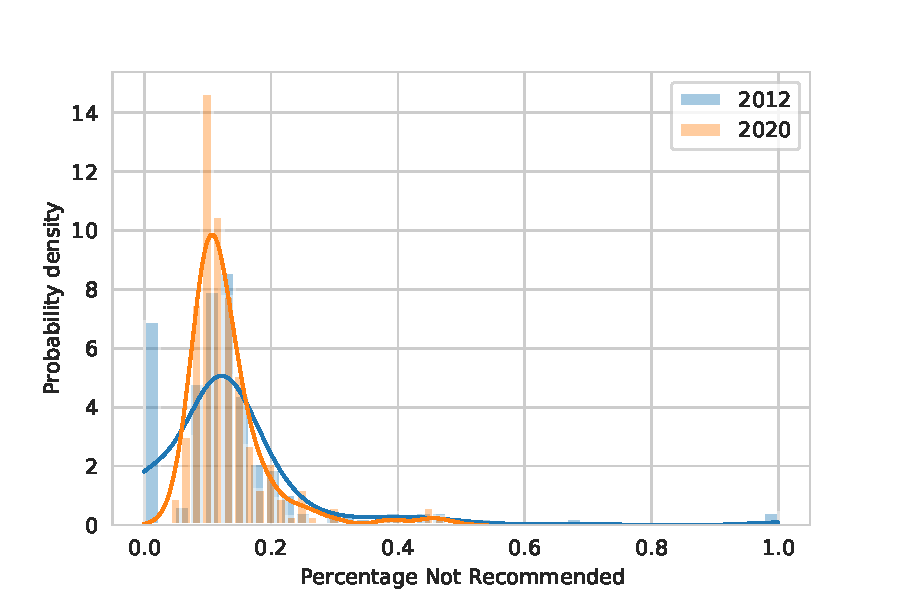
\includegraphics[width=0.9\columnwidth]{chapters/reviews/figures/filtered_proportion_density.pdf}
    \caption{Probability density of Not Recommended review percentage for a business, 2012 and 2020 data. Lines are the kernel density estimates.}
    \label{fig:filtered_density}
\end{figure}

\begin{figure}[t]
    \centering
    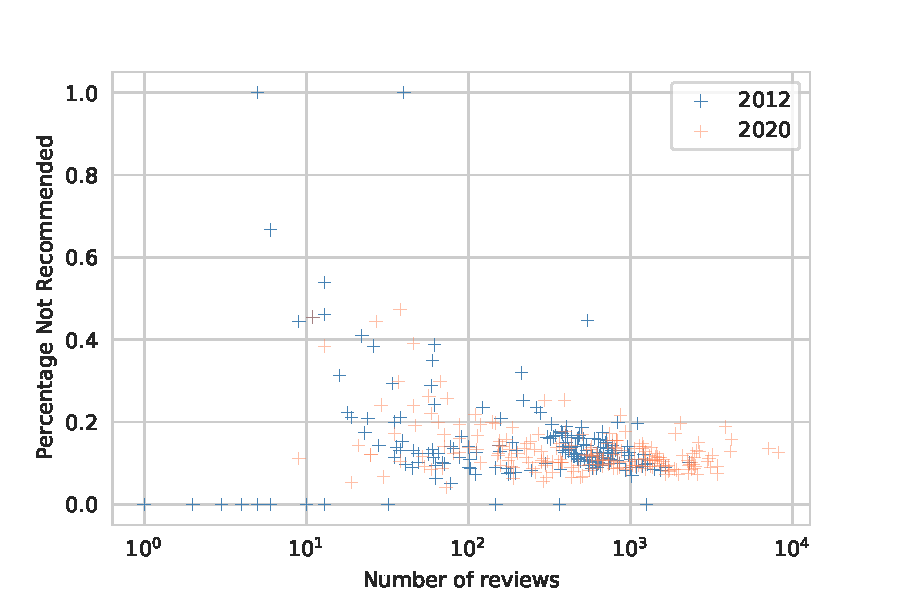
\includegraphics[width=0.9\columnwidth]{chapters/reviews/figures/filtered_vs_count.pdf}
    \caption{Number of reviews versus the percentage of reviews that were Not Recommended for a business, 2012 and 2020 data.}
    \label{fig:count_vs_perc}
\end{figure}

\textbf{The percentages of Not Recommended reviews by businesses tend to converge with more reviews.} To understand whether review classification has changed at a business level, we examined the distribution of percentage of Not Recommended reviews per businesses and the connection between number of reviews and percentage Not Recommended per business. Figure~\ref{fig:filtered_density} shows the distribution of percentage Not Recommended by business. The median percentage Not Recommended is similar (0.122 and 0.115), but the distributions are distinct (Kolmogorov–Smirnov test $\text{p}<0.01$). In the 2012, a number of business have no Not Recommended reviews. Some of these results may be explained by the business having fewer reviews in 2012 than 2020. Figure~\ref{fig:count_vs_perc} shows the connection between the number of reviews on a business and the percentage Not Recommended. Most businesses converge to around the same percentage Not Recommended with enough reviews. This convergence appears tighter among the 2020 data. We note that there is no significant correlation between the number of reviews and the percentage Recommended for the 2012 data (Spearman's correlation $\rho = 0.13$, $\text{p} = 0.06$), but there is a significant, negative correlation for the 2020 data ($\rho = -0.31$, $\text{p}<1\text{e}-5$)---the more reviews a business has, the smaller the proportion of Not Recommended reviews. The correlation for the 2020 data may be more significant because the businesses are more established.
%\rmNote{Suggested edit for above paragraph below. I tried to be a little more precise about the quantities at the cost of verbosity. Since the figures are plotted by Not Recommended reviews, I find that it's usually clearer to be consistent in the prose, especially since the semantics are equivalent. Also, I added paragraph structure to this subsection to make it clearer. If space concerns become acute, that paragraph structure can be recollapsed.}
% \textbf{The percentages of Not Recommended reviews by businesses tend to converge with more reviews.}
% To understand how reclassification has redistributed the classifications of Recommended and Not Recommended on reviews at the business level, we examine the distribution of the percentage of Not Recommended Reviews by business. We also examine the connection between the distribution of the number of reviews by business and the distribution of the percentage of those reviews that are Not Recommended.

%Figure~\ref{fig:filtered_density} shows the distributions of the percentage of Not Recommended Reviews by business observed in the two snapshots of the EYG dataset. Although the medians are similar (0.122 and 0.155 in the 2012 and 2020 snapshots, respectively), the distributions are distinct (Kolmogorov–Smirnov test $\text{p}<0.01$). In the 2012 snapshot, some businesses have zero Not Recommended reviews; this may be explained for at least some of these businesses by the observation that businesses generally had fewer reviews in 2012 than 2020.

%Figure~\ref{fig:count_vs_perc} shows the connection between the distribution of the number of reviews by business and the distribution of the percentage of those reviews that are Not Recommended in the EYG dataset. In both snapshots, it appears that the percentages of Not Recommended reviews by business converge with more reviews, and this convergence appears tighter in the 2020 snapshot. Although we observe no significant correlation between the number of reviews on a business and the percentage of those reviews that are Not Recommended in the 2012 snapshot (Spearman's correlation $\rho = 0.13$, $\text{p}>0.05$), there is a significant and negative correlation in the 2020 snapshot ($\rho = -0.31$, $\text{p}<1\text{e}-5$)---the more reviews a business has, the smaller the percentage of Not Recommended reviews is likely to be. The correlation observed in the 2020 snapshot may be more significant because the businesses are more established.

\begin{table}[t]
    \centering
    \caption{Frequency of reclassification patterns observed in Chicago data over 5 timepoints. ``R'' denotes Recommended, ``N'' denotes Not Recommended.}
    \label{tab:reclassification_patterns}
    \begin{tabular}{llr}
    \# changes & Pattern & Count \\
	 \hline
	 0 & R & 1,235,194\\
	 & N & 148,278\\
	 & \textit{Total} & 1,383,472 \\
	 \hline
	 1& R $\to$ N & 4,953\\
	 & N $\to$ R & 5,573\\
	 & \textit{Total} & 10,526\\
	 \hline
	 2& R $\to$ N $\to$ R & 706\\
	 & N $\to$ R $\to$ N & 373\\
	 & \textit{Total} & 1079\\
	 \hline
	 3+ & R $\to$ N $\to$ R $\to$ N & 60\\
	 & N $\to$ R $\to$ N $\to$ R & 75\\
	 & R $\to$ N $\to$ R $\to$ N $\to$ R & 14\\
	 & N $\to$ R $\to$ N $\to$ R $\to$ N & 15\\
	 & N $\to$ R $\to$ N $\to$ R $\to$ N $\to$ R & 2\\
	 & \textit{Total} & 157\\
	 \hline
    \end{tabular}
\end{table}

\textbf{Many reviews are reclassified, a few are reclassified frequently.} To investigate the frequency and scale of reclassification on shorter timescales we investigate reviews from the CHI dataset. Table \ref{tab:reclassification_patterns} shows how frequently reviews were reclassified. In our study period, around 0.8\% of reviews were reclassified. A small fraction of reviews undergo a substantial number of changes. This is especially interesting in light of the shorter study period and the limited number of time-points---a few reviews changed classes almost every measurement. These reviews may be cases that are particularly hard for Yelp to classify. 
%\raNote{Does this fit a markov-model pattern where we assume with x\% probability of reclassifying model?}
%\rmNote{Suggested edit for above paragraph below. I'll delimit the end of the suggestion.}
%\textbf{Many reviews are reclassified, a few are reclassified frequently.}
%To investigate the frequency and scale of reclassification on shorter timescales we examine the CHI dataset. Table \ref{tab:reclassification_patterns} shows how frequently reviews were reclassified. In our study period, we did not observe a change in the classification of most reviews, we did observe reclassification at least once on around 0.8\% of reviews, and multiple times on a small fraction of reviews. This is especially interesting in light of the shorter study period and the limited number of time-points---a few reviews were reclassified almost every measurement! These reviews may be cases that are particularly hard for Yelp to classify.

%\rmNote{End of suggested edit.}

\begin{figure}[t]
    \centering
    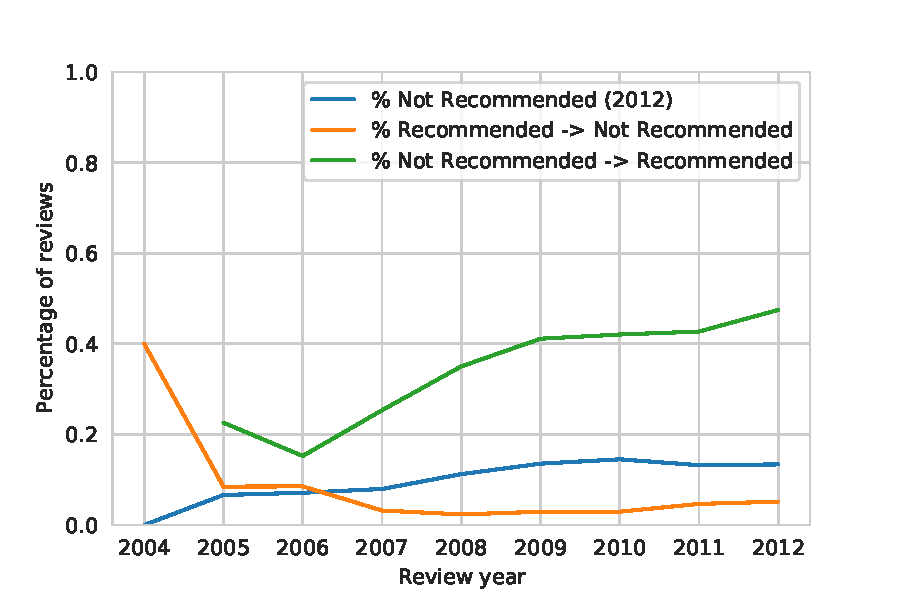
\includegraphics[width=0.9\columnwidth]{chapters/reviews/figures/filtering_changes.pdf}
    \caption{Change in recommendation status by the year reviews posted. The blue line represents reviews Not Recommended in 2012; the orange and green lines represent reviews that were Recommended and Not Recommended, respectively, in 2012 but reclassified in 2020. %\raNote{Would be good to change this to a CDF so it matches fig \ref{fig:reclassification_by_date_chicago}}
    }
    \label{fig:filtered_change}
\end{figure}

\textbf{In the long run, newer Not Recommended reviews are more likely to be reclassified.} To explore the relationship between reclassification and review age, we grouped reviews in EYG by the year posted. Within each group, we measured the percentage of reviews Yelp Recommended in 2012 and the percentage reclassified in 2020 from Recommended and Not Recommended (Figure \ref{fig:filtered_change}). Note that 2004 has just five reviews, and all were Recommended in 2012. The trend of the percentage Not Recommended in both 2012 and 2020 (green) suggests that Yelp was more likely to reclassify newer reviews from Not Recommended to Recommended. Yelp could have had more time to examine older reviews by 2012, or older, less sophisticated fake reviews may have resulted in fewer filtering errors to correct. Alternatively, this could stem from the use of review age or correlated factors (e.g., the number of reviews per author) in classification: Yelp considers whether a reviewer is ``established'' in recommending reviews~\cite{yelpwhyrec}.

\begin{figure}[t]
    \centering
    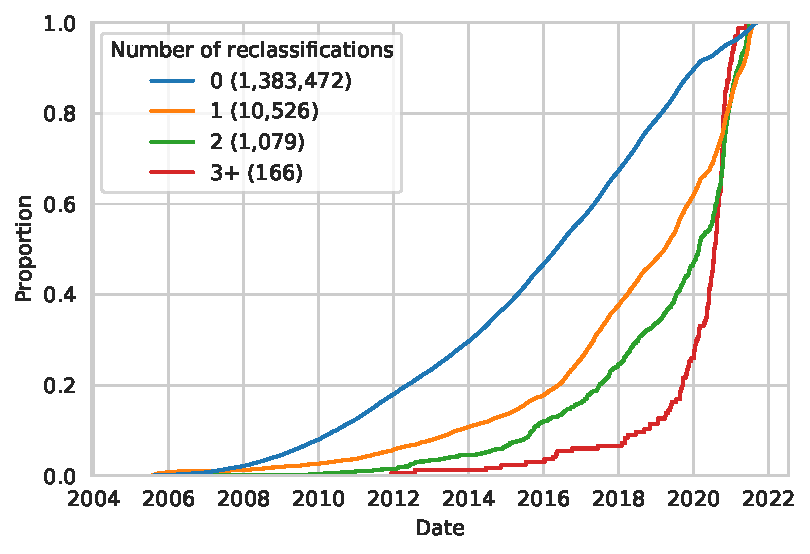
\includegraphics[width=0.9\columnwidth]{chapters/reviews/figures/reclassification_by_date_grouped_chicago.pdf}
    \caption{Cumulative percentage of reviews with a given number of reclassifications that were posted by a given date. For example, by the start of 2018 approximately 20\% of reviews with 2 observed reclassifications had been posted.}
    \label{fig:reclassification_by_date_chicago}
\end{figure}

\textbf{Newer reviews are more likely to undergo repeated reclassification, but the chance of reclassification persists over time.} Figure \ref{fig:reclassification_by_date_chicago}, shows reviews which undergo more frequent reclassification tend to be newer. This supports the idea that Yelp increases its confidence in classifying reviews as the reviews age. Perhaps because Yelp has observed more activity from the author's account or the business. We note that we still see reclassifications of reviews dating back to 2005, suggesting that a review's classification is never fully stable.
%We also see that there is little difference between the age of reviews that were reclassified zero or one times. This suggests that Yelp never fully stabilizes its classes -- even old reviews can have their classification revised.
We note a small artifact in the upper-right corner: the 1, 2, and 3+ lines rise above the 0 line. We expect this artifact because the newest reviews cannot have 1, 2, or 3+ reclassifications, since we have not made as many observations of them. These results support Yelp's statement that their classifier may mark a review as Not Recommended if it does not have sufficient data to recommend it \cite{yelprecommendationsoftware}.

Given these results showing that newer reviews are more likely to undergo reclassification and the disparity between the percentage reclassified for the EYG (8.69\% over 8 years) and CHI datasets (0.87\% over 11 months), it seems likely that Yelp's classifer is either more stable today or that Yelp performed a major overhaul between the EYG collection time-points. It's also possible that the EYG sample was disproportionately subject to reclassification.

%\raNote{I guess we could actually test this with CHI...}

% \begin{figure}[t]
%     \centering
%     \includegraphics[width=0.9\columnwidth]{figures/author_based_recommended_matching.pdf}
%     \caption{The distribution of the percentage of an author's other reviews that match the class of a given review. Reviews come from authors with two or more reviews. \raNote{Maybe there's a better way to present this. Also show reclassification instead}}
%     \label{fig:author_based_recommended_matching}
% \end{figure}

\textbf{Review classes follow the author.} In order to determine if reclassifications are performed at the author level, we investigated whether authors who have a review classifcation change are likely to have their other reviews match the new classification. In the 1,175 cases in which an author with multiple reviews had a review reclassified, 924 had all of their reviews match after reclassification. The average percentage of an author's review pairs that matched classification was 95.1\% for Recommended reviews and 94.7\% for Not Recommended reviews. This suggests that classifications follow the author.

%\raNote{ideally more analysis?}

We did not find that any particular timepoint had significantly more reclassifications.

% \raNote{maybe we can put some of the other null results here?}



% \begin{figure}[t]
%     \centering
%     \includegraphics[width=0.9\columnwidth]{figures/}
%     \caption{}
%     \label{fig:}
% \end{figure}

%Make this into a table and use constants

%0            1,305,376
%1            18,865
%2            463
%3            23
%4            1

%Non-duplicated        1324728
%Duplicated        1593

%+        1176516
%-         142541
%-+          3078
%+-          2139
%+-+          253
%-+-          177
%-+-+          15
%+-+-           8
%-+-+-          1


\subsection{Density and income impacts}

We were investigated how density and income impact reviews using our UDIS study.



\begin{figure}[t]
    \centering
    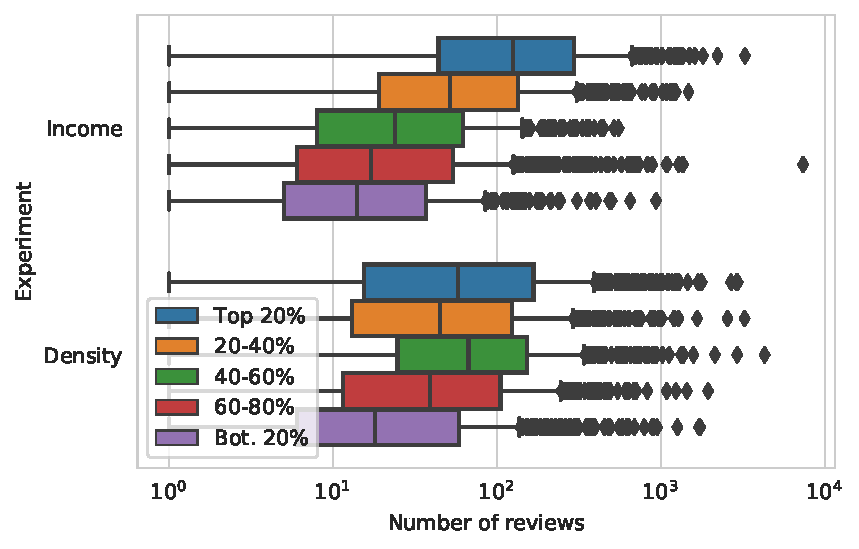
\includegraphics[width=0.9\columnwidth]{chapters/reviews/figures/reviews_per_business_stratified.pdf}
    \caption{Reviews per business. Each data point is the number of reviews for one business. }
    \label{fig:reviews_per_business_stratified}
\end{figure}

\textbf{Demographic factors correlate with the number of reviews on each business.} We investigated the number of reviews per business in Figure \ref{fig:reviews_per_business_stratified}. Both low income and low density areas have fewer reviews per business than higher income and higher density areas, and the gap is wider for density. This could be because higher income areas typically have businesses with more time on the platform---for the highest income stratum the median oldest review for each business (3,425 days) is 30\% older than for the lowest income stratum (2,638 days). This relationship is not as strong in the density experiment: the middle density stratum has the oldest reviews (3,245 days), slightly higher than the highest stratum (3,066 days) and much higher than the lowest stratum (2,704 days). The disparity in number of reviews means consumers in these areas may have less access to reviews, impacting their ability to make good decisions.

 \begin{figure}[t]
     \centering
     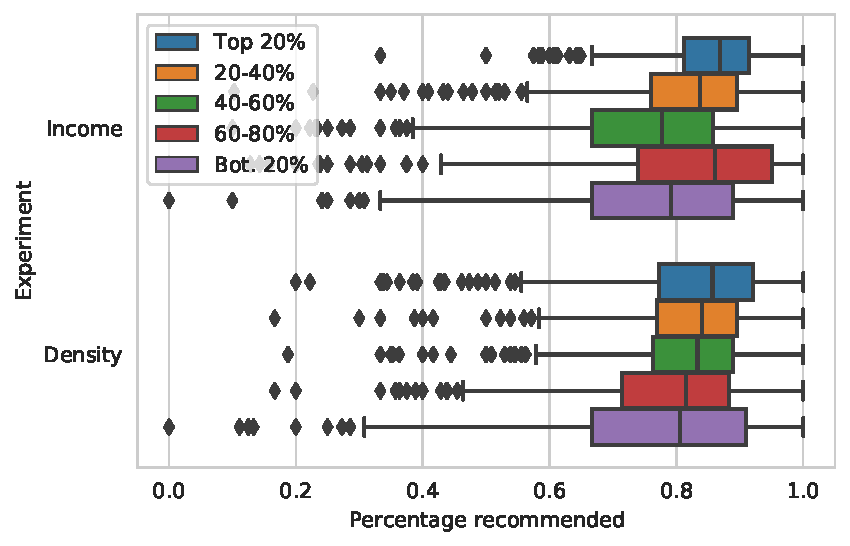
\includegraphics[width=0.9\columnwidth]{chapters/reviews/figures/percentage_recommended_per_businesses_extended.pdf}
     \caption{The proportion of reviews Recommended per business. Each data point represents one business.}
     \label{fig:percentage_recommended_per_businesses_extended}
 \end{figure}
 
\textbf{Demographic factors correlate with the percentage of reviews Recommended for each business.} We examined how the percentage of reviews that are Recommended per business varies by income and density in Figure \ref{fig:percentage_recommended_per_businesses_extended}. The range in median percentage Recommended is tighter for density---it ranges from 80\% (Bottom 20\%) to 86\% (Top 20\%)---whereas the range is larger for income, ranging from 78\% (40-60\%) to 87\% (Top 20\%). 

\begin{figure}[t]
    \centering
    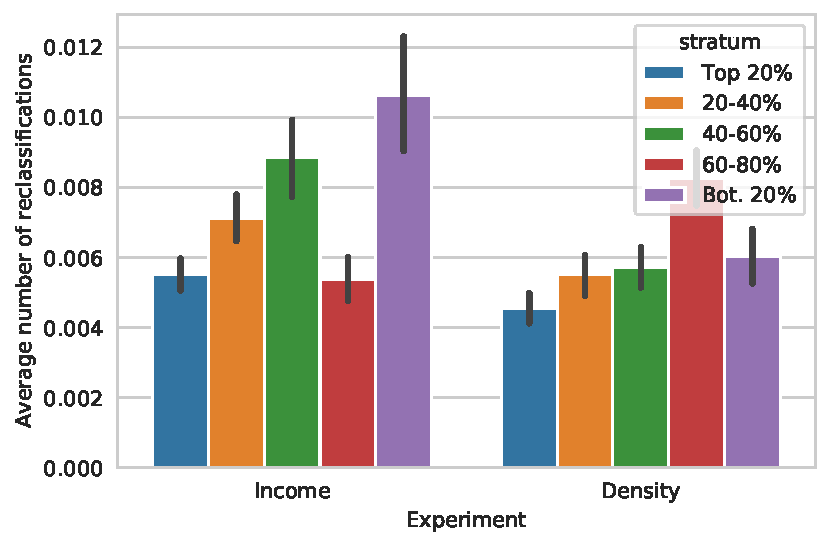
\includegraphics[width=0.9\columnwidth]{chapters/reviews/figures/stratified_reclass_swaps_usa.pdf}
    \caption{Average number of reclassifications per unique review per stratrum. Black bars indicate the 95\% confidence interval}
    \label{fig:stratified_reclass_swaps_usa}
\end{figure}

\textbf{Demographic factors correlate with the frequency of reclassifications.} In Section \ref{subsec:review_reclassification}, we explored the frequency and factors surrounding reclassification. To test whether Yelp reclassifies reviews for businesses in regions with certain income or density attributes more frequently, we looked at the average number of reclassifications per review in each stratum for both the UIS and UDS crawls (Figure \ref{fig:stratified_reclass_swaps_usa}). Less dense and lower income regions experience more reclassification. The 60-80\% strata are an outlier in both cases---the 60-80\% density stratum experiences significantly more reclassifications while the 60-80\% income stratum experiences significantly less than its neighbors, but on par with the top income stratum, which warrants further research. These disparities invite questions as to why they arise: is there something inherent about these markets that leads to more challenging-to-classify reviews, or is Yelp's classifier not well tuned to them?



\subsection{Masking}

\begin{figure}[t]
    \centering
    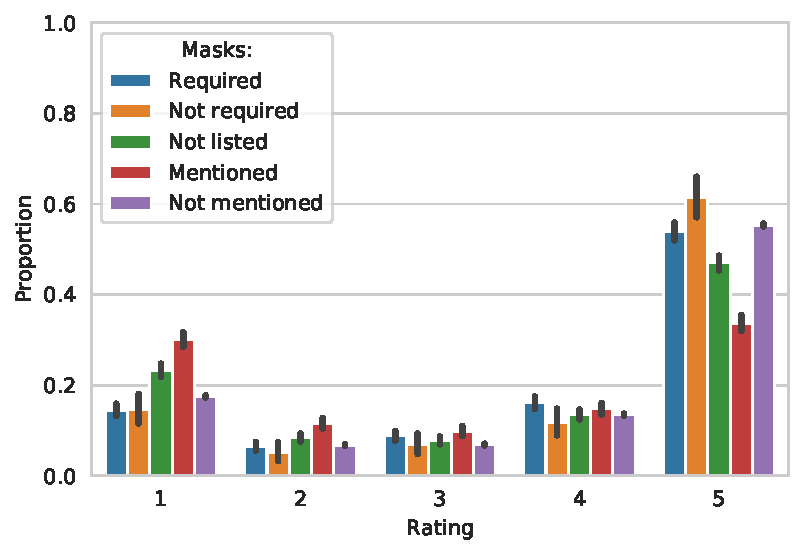
\includegraphics[width=0.9\columnwidth]{chapters/reviews/figures/proprotion_Masks_by_Rating_usa.pdf}
    \caption{The proportion by rating of reviews on or after August 06, 2021 on businesses that require/do not require/do not list a requirement for masks and reviews on or after March 1, 2020 that mention/do not mention masks. Black bars indicate the 95\% confidence interval.
    %\raNote{Update -- change order, clean up labels, y axis label}
    }
    \label{fig:proprotion_Masks mentions_masks required_by_rating_usa}
\end{figure}

In response to the COVID-19 pandemic, Yelp added an option for businesses to specify a mask policy in August 2021. Because this coincided with our longitudinal data collection, we studied reviews that mention masks and business with listed mask policies. We used our UDIS-4 crawl data because that crawl started after Yelp added the option. 

We determined whether a review mentioned masks by tokenizing the review and lemmatizing the tokens. If any lemma matched ``mask", we considered that review to mention masks. We find that 90.2\% (2,845) of UDIS reviews mentioning masks occur on or after March 1, 2020. We manually examined a random sample of 20 such reviews from before March 1, 2020; 16 of used ``mask'' to describe covering a taste or odor, 1 in a COVID-19 context, and 3 to describe costumes. We examined a random sample of 20 such reviews from on or after March 1, 2020; all 20 of them used ``mask'' in a COVID-19 context. To determine whether a business has a masking policy, we used the business amenities as described in Section \ref{subsec:crawling}. We found 837 businesses requiring masks, 174 not requiring masks, and 4,666 with no listed policy.

\textbf{Mask policies have little correlation with rating, as long as one is present. Discussions of masks correspond to lower ratings.} We show how both customer mask requirements and mask discussion affect rating in Figure \ref{fig:proprotion_Masks mentions_masks required_by_rating_usa}. Reviews mentioning masks have a lower rating, and this relationship remains after removing Not Recommended reviews. Having a mask requirement results in a slightly lower rating (means 3.89 and 4.00, Spearman correlation $\rho = -0.04$, $\text{p}<0.05$), but this relationship vanishes after removing Not Recommended reviews (mean 3.92 and 3.90, Spearman correlation $\rho = -0.01$, $\text{p}=0.79$). This suggests Yelp's filter may have the effect of protecting restaurants requiring masks. Listing any policy correlates with higher ratings; this could be explained by the overall correlation between higher ratings and more listed amenities: the Spearman's rank correlation between the rating and the number of amenities is $\rho=0.119$ $(\text{p}<<1\text{e}-5)$.   % \raNote{scipy says p=0 but that must be floating point rounding}.



